\documentclass[../../main]{subfiles}
\pagestyle{fancy}

\begin{document}

\chapter{External core model induction}
\lipsum[1]

\section{HOD mice}
\todo[inline]{Provide overview of this section.}

\subsection{Iteration strategies}

\todo[inline]{At some point we should mention that we adopt John`s convention of hiding the degree of iteration trees, always taking the maximal possible degree. And that all of our trees are (stacks of) normal trees.}

\defi{ 
  Let $\vec{\mathcal{T}}$ be a stack of normal trees. We write $\lh(\vec{\mathcal{T}})$ for the length of $\vec{\mathcal{T}}$ and $\mathcal{T}_{\alpha}$ for the $\alpha$'th tree in $\vec{\mathcal{T}}$, so that
  \eq{
    \vec{\mathcal{T}} = (\mathcal{T}_{\alpha} \mid \alpha < \lh(\vec{\mathcal{T}})).
  }

  For $\alpha < \beta < \lh(\vec{\mathcal{T}})$, $\gamma < \lh(\mathcal{T}_{\alpha})$, $\eta < \lh(\mathcal{T}_{\beta})$ we let $\mathcal{M}^{\mathcal{T}_{\alpha}}_{\gamma}$ be the model with index $\gamma$ in the tree $\mathcal{T}_{\alpha}$ and write
  \eq{
    \pi^{\vec{\mathcal{T}}}_{(\alpha, \gamma), (\beta, \eta)} \colon \mathcal{M}^{\mathcal{T}_{\alpha}}_{\gamma} \to \mathcal{M}^{\mathcal{T}_{\beta}}_{\eta}
  }

  for the corresponding embedding, provided it exists. We also write
  \eq{
    \pi^{\vec{\mathcal{T}}}_{\alpha, \beta} \colon \mathcal{M}^{\mathcal{T}_{\alpha}}_{0} \to \mathcal{M}^{\mathcal{T}_{\beta}}_{0}.
  }

  If $\vec{\mathcal{T}}$ has a last model, i.e. if $\lh(\vec{\mathcal{T}}) = \xi + 1$ and $\mathcal{M}^{\mathcal{T}_{\xi}}_{\infty}$ exists, we let $\mathcal{M}^{\vec{\mathcal{T}}}_{\infty} := \mathcal{M}^{\mathcal{T}_{\xi}}_{\infty}$ and $\pi^{\vec{\mathcal{T}}} \colon \mathcal{M}^{\mathcal{T}_{0}}_{0} \to \mathcal{M}^{\vec{\mathcal{T}}}_{\infty}$ be the associated embedding.
}


\defi{ 
  Let $\Sigma$ be an iteration strategy and $(\vec{\mathcal{T}}, N) \in I(\mathcal{M}_{\Sigma}, \Sigma)$. We write $\Sigma_{\vec{\mathcal{T}}, N}$ for the iteration strategy on $N$ given by
  \eq{
    \Sigma_{\vec{\mathcal{T}}, N}(\vec{\mathcal{U}}) := \Sigma(\vec{\mathcal{T}} ^{\frown} \vec{\mathcal{U}}).
  }

  We call $\Sigma_{\vec{\mathcal{T}}, N}$ the \textbf{$(\vec{\mathcal{T}}, N)$-tail strategy}of $\Sigma$.
}

\defi{ 
  \todo[inline]{at the very end we should remove those definitions that we didn`t need}
  Let $\Sigma$ be an iteration strategy.
  \begin{enumerate}
    \item $\Sigma$ has the \textbf{Dodd-Jensen property} if for all $(\vec{\mathcal{T}}, N) \in I(\mathcal{M}_{\Sigma}, \Sigma)$ and all $\pi \colon \mathcal{M}_{\Sigma} \to_{\Sigma_{1}} N$ we have $\pi^{\vec{\mathcal{T}}}(\alpha) \le \pi(\alpha)$ for all $\alpha \in o(\mathcal{M}_{\Sigma})$.
    \item $\Sigma$ has the \textbf{positional Dodd-Jensen property} if $\Sigma_{\vec{\mathcal{T}},N}$ has the Dodd-Jensen property for all $(\vec{\mathcal{T}},N) \in I(\mathcal{M}_{\Sigma}, \Sigma)$.
    \item $\Sigma$ is \textbf{weakly positional} if $\Sigma_{\vec{\mathcal{T}},N} = \Sigma_{\vec{\mathcal{U}},N}$ for all $(\vec{\mathcal{T}},N), (\vec{\mathcal{U}}, N) \in I(\mathcal{M}_{\Sigma}, \Sigma)$.
    \item $\Sigma$ is \textbf{positional} if $\Sigma_{\vec{\mathcal{T}}, N}$ is weakly positional for all $(\vec{\mathcal{T}}, N) \in I(\mathcal{M}_{\Sigma}, \Sigma)$.
    \item $\Sigma$ is \textbf{weakly commuting} if $\pi^{\vec{\mathcal{T}}} = \pi^{\vec{\mathcal{U}}}$ for all $(\vec{\mathcal{T}}, N), (\vec{\mathcal{U}}, N) \in I(\mathcal{M}_{\Sigma}, \Sigma)$.
    \item $\Sigma$ is \textbf{commuting} if $\Sigma_{\vec{\mathcal{T}}, N}$ is weakly commuting for all $(\vec{\mathcal{T}}, N) \in I(\mathcal{M}_{\Sigma}, \Sigma)$.
    \item $\Sigma$ is \textbf{weakly pullback consistent} if $\Sigma^{\vec{\mathcal{T}}} = \Sigma$ for all $(\vec{\mathcal{T}}, N) \in I(\mathcal{M}_{\Sigma}, \Sigma)$.
    \item $\Sigma$ is \textbf{pullback consistent} if $\Sigma_{N, \vec{\mathcal{T}}}$ is weakly pullback consistent for all $(\vec{\mathcal{T}}, N) \in I(\mathcal{M}_{\Sigma}, \Sigma)$.      
  \end{enumerate}
}

\defi{
  If $\Sigma$ is positional, $\Sigma_{\vec{\mathcal{T}}, N}$ doesn`t depend on $\vec{\mathcal{T}}$ and hence we simply write $\Sigma_{N}$ for this tail strategy.
}

\defi{ 
  An iteration strategy $\Sigma$ has \textbf{branch condensation} (see \autoref{fig:branch condensation}) if for any two stacks $\vec{\mathcal{T}}, \vec{\mathcal{U}}$ on $\mathcal{M}_{\Sigma}$ such that
  \begin{enumerate}
    \item $\vec{\mathcal{T}}, \vec{\mathcal{U}}$ are according to $\Sigma$,
    \item $\vec{\mathcal{U}}$ is a stack of successor length $\gamma + 1$ and $\vec{\mathcal{U}}$`s last component $\mathcal{U}_{\gamma}$is of limit length,
    \item $\vec{\mathcal{T}}$ has a last model $N$ such that $(\vec{\mathcal{T}}, N) \in I(\mathcal{M}_{\Sigma}, \Sigma)$,
    \item there is some branch $c$ such that $\pi^{\vec{\mathcal{U}}}_{c}$ exists and for some $\pi \colon \mathcal{M}^{\vec{\mathcal{U}}}_{c} \to_{\Sigma_{1}} N$ we have $\pi^{\vec{\mathcal{T}}} = \pi \circ \pi^{\vec{\mathcal{U}}}_{c}$.\\
  \end{enumerate}

  Then $c = \Sigma(\vec{\mathcal{U}})$.
}

\begin{figure}
  \centering
  \begin{tikzcd}[row sep=large, column sep=large] & & N \\
    \mathcal{M}_{\Sigma} \arrow[urr, "\pi^{\vec{\mathcal{T}}}"] \arrow[drr, "\pi^{\vec{\mathcal{U}}}_{c}"]& & \\ & & \mathcal{M}^{\vec{\mathcal{U}}}_{c} \arrow[uu, "\pi"]
  \end{tikzcd}
  \caption{Branch condensation}
  \label{fig:branch condensation}
\end{figure}

\defi{
  % Caution: % $(\mathcal{M}, \mathcal{T}), (\mathcal{N}, \mathcal{U})$ are % flipped when compared to Grigor`s thesis Let $\mathcal{M}, \mathcal{N}$ be layered hybrid premice and $\mathcal{T}, \mathcal{U}$ be normal trees on $\mathcal{M}, \mathcal{N}$ respectively.
  \textbf{$(\mathcal{M}, \mathcal{T})$ is a hull of $(\mathcal{N}, \mathcal{U})$} if there are
  \begin{enumerate}
    \item an embedding, $\pi \colon \mathcal{M} \to_{\Sigma_{1}} \mathcal{N}$ and
    \item an order-preserving map $\sigma \colon \lh(\mathcal{T}) \to \lh(\mathcal{U})$
  \end{enumerate}

  such that
  \begin{enumerate}
    \item $\alpha \le_{\mathcal{T}} \beta \iff \sigma(\alpha) \le_{\mathcal{U}} \sigma(\beta)$
    \item $[\alpha,\beta]_{\mathcal{T}} \cap \mathcal{D}^{\mathcal{T}} = \emptyset \iff [\sigma(\alpha),\sigma(\beta)]_{\mathcal{U}} \cap \mathcal{D}^{\mathcal{U}} = \emptyset$,
    \item $\pi_{\alpha} \colon \mathcal{M}_{\alpha}^{\mathcal{T}} \to \mathcal{M}_{\sigma(\alpha)}^{\mathcal{U}}$ and $\pi_{\alpha}(E^{\mathcal{T}}_{\alpha}) = E^{\mathcal{U}}_{\sigma(\alpha)}$,
    \item for $\beta < \alpha$ we have $\pi_{\alpha} \restriction \lh(E_{\beta}^{\mathcal{T}}) + 1 = \pi_{\beta} \restriction \lh(E_{\beta}^{\mathcal{T}}) + 1$,
    \item for $\alpha \le_{\mathcal{T}} \beta$ with $[\alpha,\beta]_{\mathcal{T}} \cap \mathcal{D}^{\mathcal{T}}$ we have $\pi_{\beta} \circ \pi^{\mathcal{T}}_{\alpha,\beta} = \pi^{\mathcal{U}}_{\sigma(\alpha), \sigma(\beta)} \circ \pi_{\alpha}$,
      \item if $\beta = \pred_{\mathcal{T}}(\alpha + 1)$, then $\sigma(\beta) = \pred_{\mathcal{U}}(\sigma(\alpha + 1))$ and $\pi_{\alpha+1}([a,f]_{E^{\mathcal{T}}_{\alpha}}) = [\pi_{\alpha}(a), \pi_{\beta}(f)]_{E^{\mathcal{T}}_{\sigma(\alpha)}}$ and
    \item $0 \le_{\mathcal{U}} \sigma(0)$, $[0, \sigma(0)] \cap \mathcal{D}^{\mathcal{U}} = \emptyset$ and $\pi_{0} = \pi^{\mathcal{U}}_{0, \sigma(0)} \circ \pi$,
  \end{enumerate}
  (See \autoref{fig:hull of U})
}

\defi{ 
  Let $\mathcal{M}, \mathcal{N}$ be layered hybrid premice and $\vec{\mathcal{T}}, \vec{\mathcal{U}}$ be stacks of normal trees on $\mathcal{M}, \mathcal{N}$ respectively.
  \textbf{$(\mathcal{M}, \vec{\mathcal{T}})$ is a hull of $(\mathcal{N}, \vec{\mathcal{U}})$} \label{hull of a stack of normal trees} if there are
  \begin{enumerate}
    \item an order presercing map $\sigma \colon \lh(\vec{\mathcal{T}}) \to \lh(\vec{\mathcal{U}})$,
    \item a sequence $(\sigma_{\alpha} \mid \alpha < \lh(\vec{\mathcal{T}}))$ of order preserving maps $\sigma_{\alpha} \colon \lh(\mathcal{T}_{\alpha}) \to \lh(\mathcal{U}_{\sigma(\alpha)})$,
    \item $(\pi_{\alpha,\beta} \mid \alpha < \lh(\vec{\mathcal{T}}) \wedge \beta < \lh(\mathcal{T}_{\alpha}))$ such that
      \begin{enumerate}
        \item $\pi_{0,0} = \pi^{\vec{\mathcal{U}}}_{0, \sigma(0)}$ (so that $\pi_{0,0} = \id$ if $\sigma(0) = 0$),
        \item for $\alpha < \lh(\vec{\mathcal{T}})$
          \eq{
            \pi_{\alpha,0} \colon \mathcal{M}_{\alpha}^{\vec{\mathcal{T}}} \to_{\Sigma_{1}} \mathcal{M}^{\vec{\mathcal{U}}}_{\sigma(\alpha)}
          }
          and $(\mathcal{M}^{\vec{\mathcal{T}}}_{\alpha}, \mathcal{T}_{\alpha})$ is a $(\pi_{\alpha,0}, \sigma_{0})$-hull of $(\mathcal{M}^{\vec{\mathcal{U}}}_{\sigma(\alpha)}, \mathcal{U}_{\sigma(\alpha)})$,
        \item $\alpha < \beta < \lh(\vec{\mathcal{T}})$ and $\pi^{\vec{\mathcal{T}}}_{(\alpha,\gamma), (\beta, \eta)}$ exists, then $\pi^{\vec{\mathcal{U}}}_{(\sigma(\alpha), \sigma_{\alpha}(\gamma)), (\sigma(\beta), \sigma_{\beta}(\eta))}$ exists and
          \eq{
            \pi_{\beta,\eta} \circ \pi^{\vec{\mathcal{T}}}_{(\alpha,\gamma), (\beta,\eta)} = \pi^{\vec{\mathcal{U}}}_{(\sigma(\alpha), \sigma_{\alpha}(\gamma)), (\sigma(\beta), \sigma_{\beta}(\eta))} \circ \pi_{\alpha, \gamma}.
          }
      \end{enumerate}
  \end{enumerate}
  (See \autoref{fig:hull of stack of normal tree})
}

\begin{figure}
  \centering % 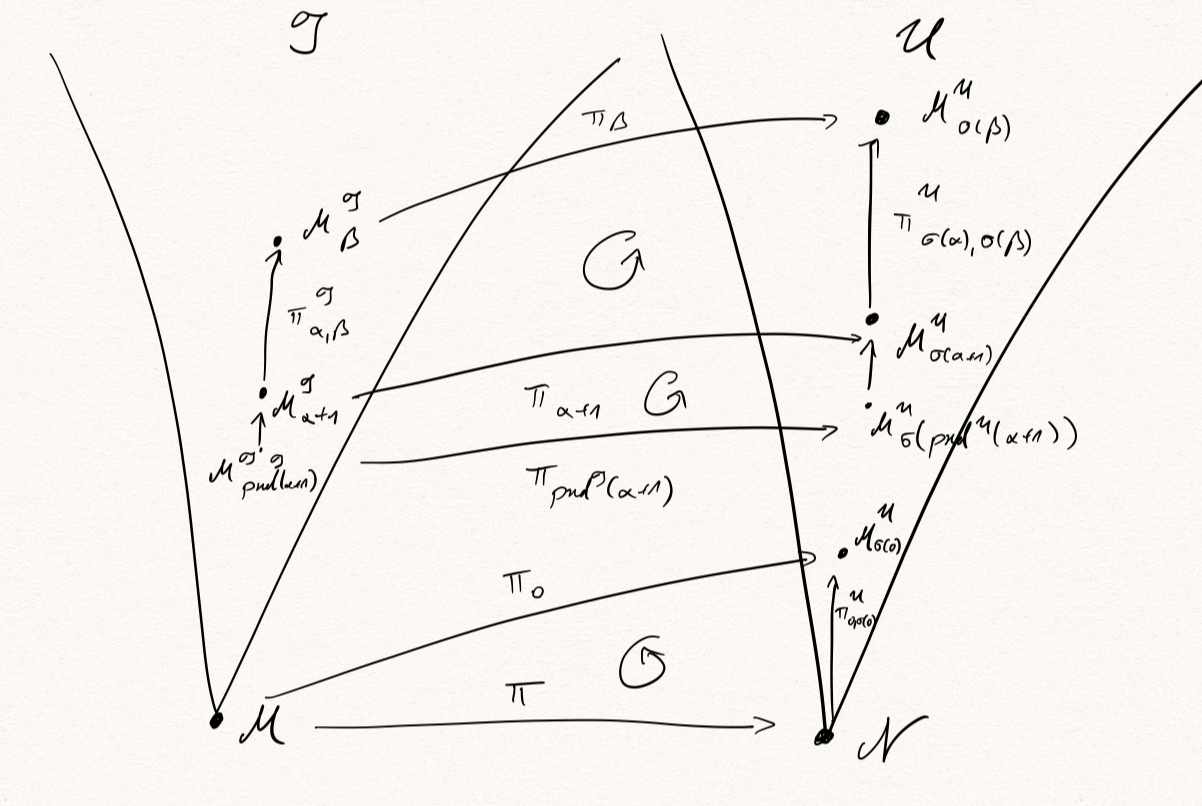
\includegraphics[width=300px]{\string~/gitsky/phd/gfx/hull-of-U.png}
  \begin{tikzpicture}
    \coordinate (rootl) at (0,0);
    \coordinate (rootr) at (7,0);
    
    \coordinate (treel) at (-2,7);
    \coordinate (treer) at (2,7);

    \coordinate (modelroot) at (0,0);
    \coordinate (modelroottarget) at (0,1.5);
    \coordinate (model0) at (0,2.5);
    \coordinate (model1) at (0,4);
    \coordinate (model2) at (0,6);
    \coordinate (offsetr) at (0,1);

    \draw [dotted] (rootl) -- ($(rootl) + (treel)$);
    \draw [dotted] (rootl) -- ($(rootl) + (treer)$);

    \draw [dotted] (rootr) -- ($(rootr) + (treel) + (offsetr)$);
    \draw [dotted] (rootr) -- ($(rootr) + (treer) + (offsetr)$);

    % models of left tree
    \fill ($(rootl) + (modelroot)$) circle[radius=1pt] node[left]
    {$\mathcal{M}^{\mathcal{T}}_{0}$};
    \fill ($(rootl) + (model0)$) circle[radius=1pt] node[left]
    {$\mathcal{M}^{\mathcal{T}}_{\pred^{\mathcal{T}}(\alpha+1)}$};
    \fill ($(rootl) + (model1)$) circle[radius=1pt] node[left]
    {$\mathcal{M}^{\mathcal{T}}_{\alpha+1}$};
    \fill ($(rootl) + (model2)$) circle[radius=1pt] node[left]
    {$\mathcal{M}^{\mathcal{T}}_{\beta}$};

    % models of right tree
    \fill ($(rootr) + (modelroot)$) circle[radius=1pt] node[right]
    {$\mathcal{M}^{\mathcal{U}}_{0}$};
    \fill ($(rootr) + (modelroottarget)$) circle[radius=1pt] node[right]
    {$\mathcal{M}^{\mathcal{U}}_{\sigma(0)}$};
    \fill ($(rootr) + (model0) + (offsetr)$) circle[radius=1pt] node[right]
    {$\mathcal{M}^{\mathcal{U}}_{\sigma(\pred^{\mathcal{T}}(\alpha+1))}$};
    \fill ($(rootr) + (model1) + (offsetr)$) circle[radius=1pt] node[right]
    {$\mathcal{M}^{\mathcal{U}}_{\sigma(\alpha+1)}$};
    \fill ($(rootr) + (model2) + (offsetr)$) circle[radius=1pt] node[right]
    {$\mathcal{M}^{\mathcal{U}}_{\sigma(\beta)}$};

    % embeddings between trees
    \draw [->] ($(rootl) + (modelroot)$) -- node[below]{$\pi$}($(rootr) + (modelroot)$);
    \draw [->] ($(rootl) + (modelroot)$) -- node[above]{$\pi_{0}$}($(rootr) + (modelroottarget)$);
    \draw [->] ($(rootr) + (modelroot)$) -- node[right]{$\pi^{\mathcal{U}}_{0, \sigma(0)}$} ($(rootr) + (modelroottarget)$);

    \draw [->] ($(rootl) + (model0)$) -- node[below]{$\pi_{\pred^{\mathcal{T}}(\alpha+1)}$} ($(rootr) + (model0) + (offsetr)$);
    \draw [->] ($(rootl) + (model1)$) -- node[below]{$\pi_{\alpha+1}$} ($(rootr) + (model1) + (offsetr)$);
    \draw [->] ($(rootl) + (model2)$) -- node[below]{$\pi_{\beta}$} ($(rootr) + (model2) + (offsetr)$);

    % embeddings in left tree
    \draw [->] ($(rootl) + (model0)$) -- node[right]{$\pi^{\mathcal{T}}_{\pred^{\mathcal{T}}(\alpha+1), \alpha+1}$}($(rootl) + (model1)$);
    \draw [->] ($(rootl) + (model1)$) -- node[right]{$\pi^{\mathcal{T}}_{\alpha+1, \beta}$}($(rootl) + (model2)$);

    % embeddings in right tree
    \draw [->] ($(rootr) + (model0) + (offsetr)$) -- node[right]{$\pi^{\mathcal{U}}_{\sigma(\pred^{\mathcal{T}}(\alpha+1)), \sigma(\alpha+1)}$}($(rootr) + (model1) + (offsetr)$);
    \draw [->] ($(rootr) + (model1) + (offsetr)$) -- node[right]{$\pi^{\mathcal{U}}_{\sigma(\alpha+1), \sigma(\beta)}$}($(rootr) + (model2) + (offsetr)$);
  \end{tikzpicture}
  \caption{$\mathcal{T}$ is a hull of $\mathcal{U}$}
  \label{fig:hull of U}
\end{figure}

\begin{figure}
  \centering % placeholder % 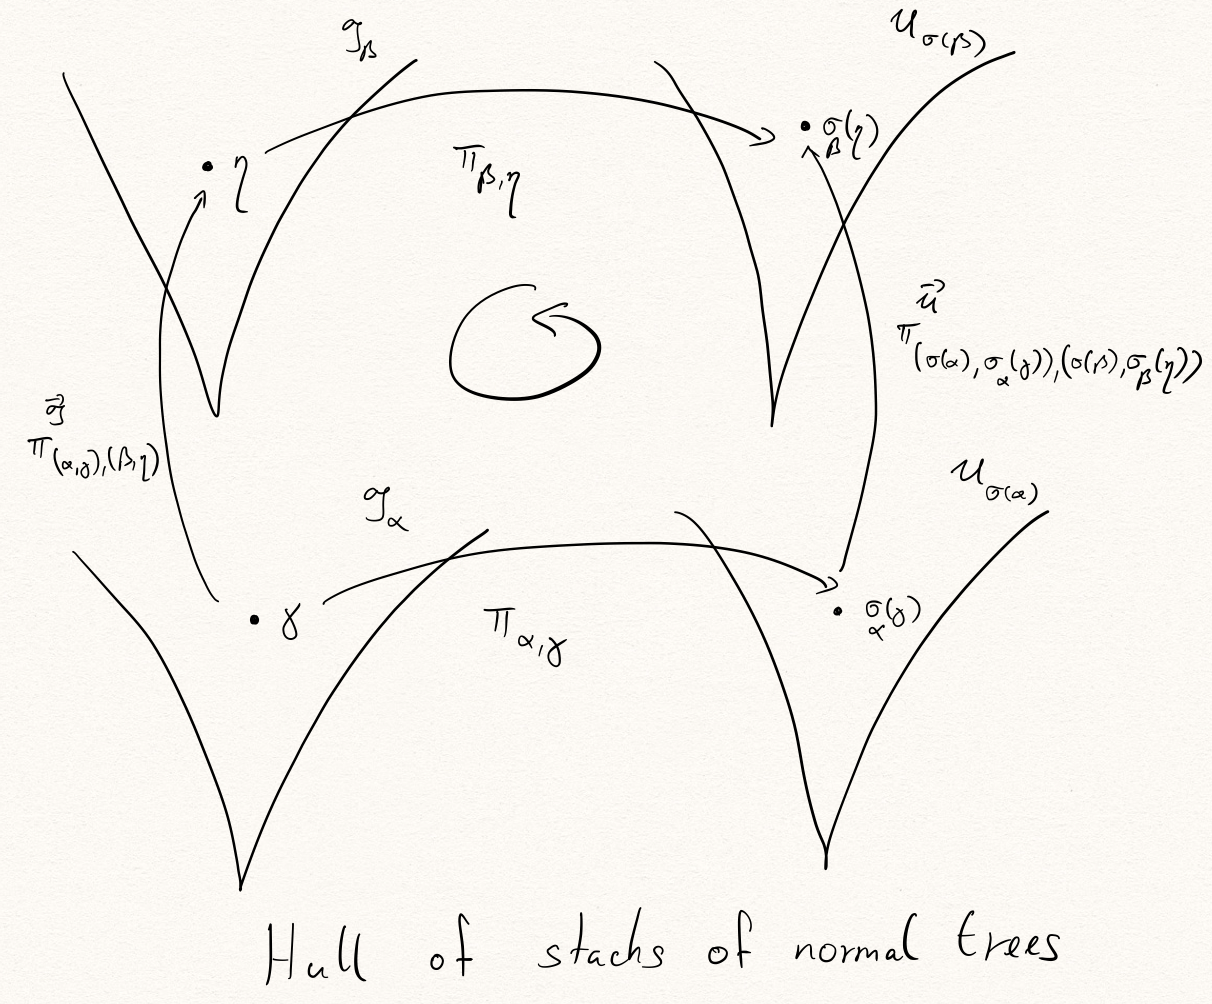
\includegraphics[width=300px]{\string~/gitsky/phd/gfx/hull-of-vec-U.png}
  \begin{tikzpicture}
    \coordinate (rootul) at (0,0);
    \coordinate (rootur) at (5,1);
    \coordinate (rootdl) at (0,-4);
    \coordinate (rootdr) at (5,-3);
    
    \coordinate (treel) at (-2,3);
    \coordinate (treer) at (2,3);
    \coordinate (model) at (0,2);

    % Tree upper left
    \draw (rootul) node[below]{$\mathcal{T}_{\beta}$} -- ($(rootul) + (treel)$);
    \draw (rootul) -- ($(rootul) + (treer)$);
    \fill ($(rootul) + (model)$) circle[radius=1pt] node[below right]
    {$\mathcal{M}^{\mathcal{T}_{\beta}}_{\eta}$};

    % Tree upper right
    \draw (rootur) node[below]{$\mathcal{U}_{\sigma(\beta)}$} -- ($(rootur) + (treel)$);
    \draw (rootur) -- ($(rootur) + (treer)$);
    \fill ($(rootur) + (model)$) circle[radius=1pt] node[right]
    {$\mathcal{M}^{U_{\sigma(\beta)}}_{\sigma_{\beta}(\eta)}$};

    % Tree down left
    \draw (rootdl) node[below]{$\mathcal{T}_{\alpha}$} -- ($(rootdl) + (treel)$);
    \draw (rootdl) -- ($(rootdl) + (treer)$);
    \fill ($(rootdl) + (model)$) circle[radius=1pt] node[below right]
    {$\mathcal{M}^{T_{\alpha}}_{\gamma}$};

    % Tree down right
    \draw (rootdr) node[below]{$\mathcal{U}_{\sigma(\alpha)}$} -- ($(rootdr) + (treel)$);
    \draw (rootdr) -- ($(rootdr) + (treer)$);
    \fill ($(rootdr) + (model)$) circle[radius=1pt] node[right]
    {$\mathcal{M}^{U_{\sigma(\alpha)}}_{\sigma_{\alpha}(\gamma)}$};

    % Embedding left
    \draw [->] ($(rootdl) + (model)$) to [out=135,in=225] node[left]{$\pi^{\vec{\mathcal{T}}}_{(\alpha,\gamma),(\beta,\eta)}$}
    ($(rootul) + (model)$);

    % Embedding right
    \draw [->] ($(rootdr) + (model)$) to [out=45,in=315] node[right]{$\pi^{\vec{\mathcal{U}}}_{(\sigma(\alpha),
        \sigma_{\alpha}(\gamma)), (\sigma(\beta),
        \sigma_{\beta}(\eta))}$}($(rootur) + (model)$);

    % Embedding up
    \draw [->] ($(rootul) + (model)$) to node[above]{$\pi_{\beta,\eta}$}
    ($(rootur) + (model)$);

    % Embedding down
    \draw [->] ($(rootdl) + (model)$) to node[above]{$\pi_{\alpha,\gamma}$} ($(rootdr) + (model)$);
  \end{tikzpicture}
  \caption{$\vec{\mathcal{T}}$ is a hull of $\vec{\mathcal{U}}$}
  \label{fig:hull of stack of normal tree}
\end{figure}

\defi{ 
  Let $\mathcal{M}$ be a layered hybrid premouse and $\Sigma$ be a (partial) iteration strategy for $\mathcal{M}$. $\Sigma$ has \textbf{hull condensation} if the following holds true for any two stacks $\vec{\mathcal{T}}, \vec{\mathcal{U}}$ on $\mathcal{M}$. If $\vec{\mathcal{U}}$ is according to $\Sigma$ and $\vec{\mathcal{T}}$ is a hull of $\vec{\mathcal{U}}$, then $\vec{\mathcal{T}}$ is according to $\Sigma$.
}

\lemm{ 
  Let $\Sigma$ be an iteration strategy. Then the following hold true.
  \begin{enumerate}
    \item If $\Sigma$ has hull condensation then it is pullback consistent.
    \item If $\Sigma$ is positional and pullback consistent then it is commuting.
  \end{enumerate}
}
\proof{
  See \cite[Proposition~2.36]{sargsyan2015hod}.
}


\subsection{Layered hybrid mice}

\todo[inline]{Define strategy mice as a particular kind of hybrid mice, hod mice/pairs and put in positional and commuting in the definition, state comparison. Introduce derived models of hod mice and how they relate to the Solovay hierarchy. Define $\Sigma$-mouse}

\defi{ 
  Let $\mathcal{M}$ be a transitive set (or structure). We let $o(\mathcal{M}) := \mathcal{M} \cap \on$ be the ordinal height of $\mathcal{M}$.
}

\defi{ 
  Let $\mathcal{M}$ be a (hybrid) premouse and $\alpha \le o(\mathcal{M})$. We let
  \begin{enumerate}
    \item $\mathcal{M} || \alpha$ be the initial segment of $\mathcal{M}$ of height $\alpha$ including its top extender and
    \item $\mathcal{M} | \alpha$ be the passive initial segment of $\mathcal{M}$ of height $\alpha$, i.e. $\mathcal{M} || \alpha$ but without the top extender.
  \end{enumerate}
}

\defi{ 
  Let $\mathcal{M}$ be a $\mathcal{J}$-structure \footnote{See \cite{zeman2011inner} for the basics on $\mathcal{J}$-structures, premice and their fine structure.} and $\alpha \le o(\mathcal{M})$. We write $\mathcal{J}^{\mathcal{M}}_{\alpha}$ for the $\alpha$th level of $\mathcal{M}$`s construction.
}

\defi{ 
  A \textbf{potential layered hybrid premouse} (over $X$) is an acceptable $\mathcal{J}$-structure of the form $\mathcal{M} = (J^{\vec{E},f}_{\alpha}(X); \in, \vec{E}, B, f)$ $X$ such that
  \begin{enumerate}
    \item $\vec{E}$ is a fine extender sequence (over $X$),
    \item $f$ is a function with domain $Y \subseteq \alpha$ such that $f(\gamma)$, for each $\gamma \in Y$, is a shift of an amenable function that typically codes part of an iteration strategy for $\mathcal{M}$,
  \end{enumerate}

  We will often write $\vec{E}^{\mathcal{M}}, f^{\mathcal{M}}, Y^{\mathcal{M}}$ for $\vec{E},f,Y$ as above. If all proper initial segments of $\mathcal{M}$ are sound, we say that $\mathcal{M}$ is a \textbf{layered hybrid premouse}. 
}

In our case, assuming $X$ is a self-well-ordered set, $Y^{\mathcal{M}}$ is determined by the \textbf{standard indexing scheme}
(see \cite[Definition~1.18]{sargsyan2015hod}).

%%%%%%%%%%%%%%%%%% For more details, see \cite{sargsyan2015hod}. %%%%%%%%%%%%%%%%%%

\defi{ 
  Let $\Sigma$ be a strategy for a layered hybrid premouse $\mathcal{M}$. For $\alpha \le o(M)$ we let $\Sigma_{\mathcal{M} | \alpha}$ be the $\id$-pullback iteration strategy on $\mathcal{M} | \alpha$ induced by $\Sigma$, i.e. a stack $\vec{\mathcal{T}}$ on $\mathcal{M} | \alpha$ is according to $\Sigma_{\mathcal{M} | \alpha}$ iff $\id \vec{\mathcal{T}}$ on $\mathcal{M}$, given by the copy construction via $\id$ (see \cite[4.1]{steel2010outline}), is according to $\Sigma$.
}

\defi{ 
  A \textbf{layered strategy premouse} $\mathcal{M}$ is a layered hybrid premouse such that
  \begin{enumerate}
    \item $f^{\mathcal{M}}(\gamma)$ codes a partial iteration strategy $\Sigma^{\mathcal{M}}_{\gamma}$ for $\mathcal{M} | \gamma$ and
    \item For $\gamma_{0}, \gamma_{1} \in Y^{\mathcal{M}}$, if $\gamma_{0} < \gamma_{1}$ then $(\Sigma^{\mathcal{M}}_{\gamma_{1}})_{\mathcal{M} | \gamma_{0}} \subseteq \Sigma^{\mathcal{M}}_{\gamma_{0}}$.    
  \end{enumerate}

  We also write $\Sigma^{\mathcal{M}}$ for the the strategy coded by $f^{\mathcal{M}}$.
}

\defi{
  Let $\mathcal{M}$ be a layered strategy premouse and $\Sigma$ be an iteration strategy for $\mathcal{M}$. $\mathcal{M}$ is a \textbf{$\Sigma$-premouse} if $\Sigma^{\mathcal{M}} \subseteq \Sigma$.
}

\defi{
  Let $\Sigma$ be an iteration strategy. We write $\mathcal{M}_{\Sigma}$ for the (layered hybrid) premouse $\mathcal{N}$ such that $\Sigma$ is an iteration strategy for $\mathcal{N}$.  We also let $I(\M_\Sigma, \Sigma)$ be the set of pairs $(\vec\T, N)$ such that $\vec\T$ is a stack of normal trees on $\M_\Sigma$ according to $\Sigma$, $\pi^{\vec\T}$ exists and $N$ is the last model of $\vec\T$. We also let
  \eq{
    pI(\mathcal{M}_{\Sigma}, \Sigma) := \{ N \mid \exists \vec{\mathcal{T}} \colon (\vec{\mathcal{T}}, N) \in I(\mathcal{M}_{\Sigma}, \Sigma) \}.
  }
}

\defi{ 
  A $\Sigma$-premouse $\mathcal{M}$ is a \textbf{$\Sigma$-mouse} if there is a $\omega_{1}+1$-iteration strategy $\Lambda$ such that all $\mathcal{N} \in pI(\mathcal{M}, \Lambda)$, $\mathcal{N}$ are themselves $\Sigma$-premice.
}

\defi{ 
  Let $a$ be a transitive self-well-ordered set and let $\Sigma$ be an iteration strategy with hull-condensation such that $\mathcal{M}_{\Sigma} \in a$ and let $\Gamma$ be a pointclass which is closed under Boolean operations and continuous images and preimages. Define the $(\Gamma, \Sigma)$-$\lp$ stack over $a$ recursively as follows:
  \begin{enumerate}
    \item $\lp^{\Gamma, \Sigma}_{0}(a) := a \cup \{ a \}$,
    \item $\lp^{\Gamma, \Sigma}_{\alpha + 1}(a)$ is the union of all sound $\Sigma$-mice over $\lp^{\Gamma, \Sigma}_{\alpha}(a)$ that projects to $o(\lp^{\Gamma, \Sigma}_{\alpha}(a))$ and which has an iteration strategy in $\Gamma$,
    \item $\lp^{\Gamma, \Sigma}_{\lambda}(a) := \bigcup_{\alpha < \lambda} \lp^{\Gamma, \Sigma}(a)$ for limit $\lambda$.
  \end{enumerate}

  We also let $\lp^{\Gamma, \Sigma}(a) := \lp^{\Gamma, \Sigma}_{1}(a)$.
}

\subsection{HOD mice}

\defi[][defi:hod premouse]{
  Suppose $\mathcal{P} = (J^{\vec{E},f}(X); \in, \vec{E}, f, B)$ is a layered strategic premouse. $\mathcal{P}$ is a \textbf{$\hod$-premouse}\footnote{These are in fact $\hod$-premice below $\godel{\ad_{\mathbb{R}} + \Theta \text{ is measurable}}$ in \cite{sargsyan2015hod}. However, since all of our $\hod$-mice are of this form, we omit this. } provided the following hold:
  Let $\lambda = \otp(Y^{\mathcal{P}})$, $(\gamma_{\beta} \mid \beta < \lambda)$ be the strictly increasing enumeration of $Y^{\mathcal{P}}$ and let, for $\beta < \lambda$, $\mathcal{P}(\beta) := \mathcal{P} || \gamma_{\beta}$ and moreover $\mathcal{P}(\lambda) := \mathcal{P}$. Then there is a continuous, strictly increasing sequence $(\delta_{\beta} \mid \beta \le \lambda)$ of $\mathcal{P}$-cardinals such that
  \begin{enumerate}
    \item $B = \emptyset$,
    \item $Y^{\mathcal{P}} \subseteq \delta_{\lambda}$,
    \item $(\delta_{\beta} \mid \beta \le \lambda)$ is sequence of Woodin cardinals and their limits in $\mathcal{P}$ and
    \item for all $\beta \le \lambda$

      \begin{enumerate}      
        \item $\delta_{\beta}$ is a strong cutpoint \todo{define strong cutpoint} of $\mathcal{P}$,
        \item $\mathcal{P}(\beta) \models \godel{\zfc\text{-Replacement}}$,
        \item $\mathcal{P}(\beta) = \mathcal{O}^{\mathcal{P}, \omega}_{\delta_{\beta}}$ \footnote{see \cite[Definition~1.26]{sargsyan2015hod}},
        \item if $\beta$ is a limit then $\delta_{\beta}^{+\mathcal{P}} = \delta_{\beta}^{+\mathcal{P}(\beta)}$,
        \item if $\beta < \lambda$ then $f(\gamma_{\beta})$ codes a $(o(\mathcal{P}), o(\mathcal{P}))$-strategy, call it $\Sigma^{\mathcal{P}}_{\beta}$, for $\mathcal{P}(\beta)$ with hull condensation \footnote{note that $\Sigma^{\mathcal{P}}_{\beta} \subseteq \mathcal{P}$ is an internal strategy, i.e. only defined on trees that are elements of $\mathcal{P}$},
        \item \label{defi:agreement of internal iteration strategy} if $\alpha < \beta < \lambda$, then $(\Sigma^{\mathcal{P}}_{\beta})_{\mathcal{P(\alpha)}} =
          \Sigma^{\mathcal{P}}_{\alpha}$, \todo{confirm with Grigor that this is what he had in mind}
        \item if $\beta < \lambda$ and $\eta \in (\delta_{\beta}, \delta_{\beta+1})$ is a $\mathcal{P}$-successor cardinal, then $\mathcal{P} | \eta$ is a $\Sigma^{\mathcal{P}}_{\gamma_{\beta}}$-premouse over $\mathcal{P}(\beta)$ which is $(o(\mathcal{P}), o(\mathcal{P}))$-iterable for stacks above $\delta_{\beta}$.
      \end{enumerate}

    \item $\forall n < \omega \colon \mathcal{P} \models
      \delta_{\lambda}^{+n} \text{ exists}$ and $o(\mathcal{P}) = \sup_{n < \omega}
      (\delta_{\lambda}^{+n})^{\mathcal{P}}$.
  \end{enumerate}

  See \autoref{fig:hod-premouse}. We will often write $\delta^{\mathcal{P}}_{\beta}, \gamma_{\beta}^{\mathcal{P}}, \lambda^{\mathcal{P}}$ for $\delta_{\beta}, \gamma_{\beta}, \lambda$ as above and moreover let $\delta^{\mathcal{P}} := \delta_{\lambda}$.  \todo{include an intuitive description of $\hod$-mice}
}

\begin{figure}
  \centering
  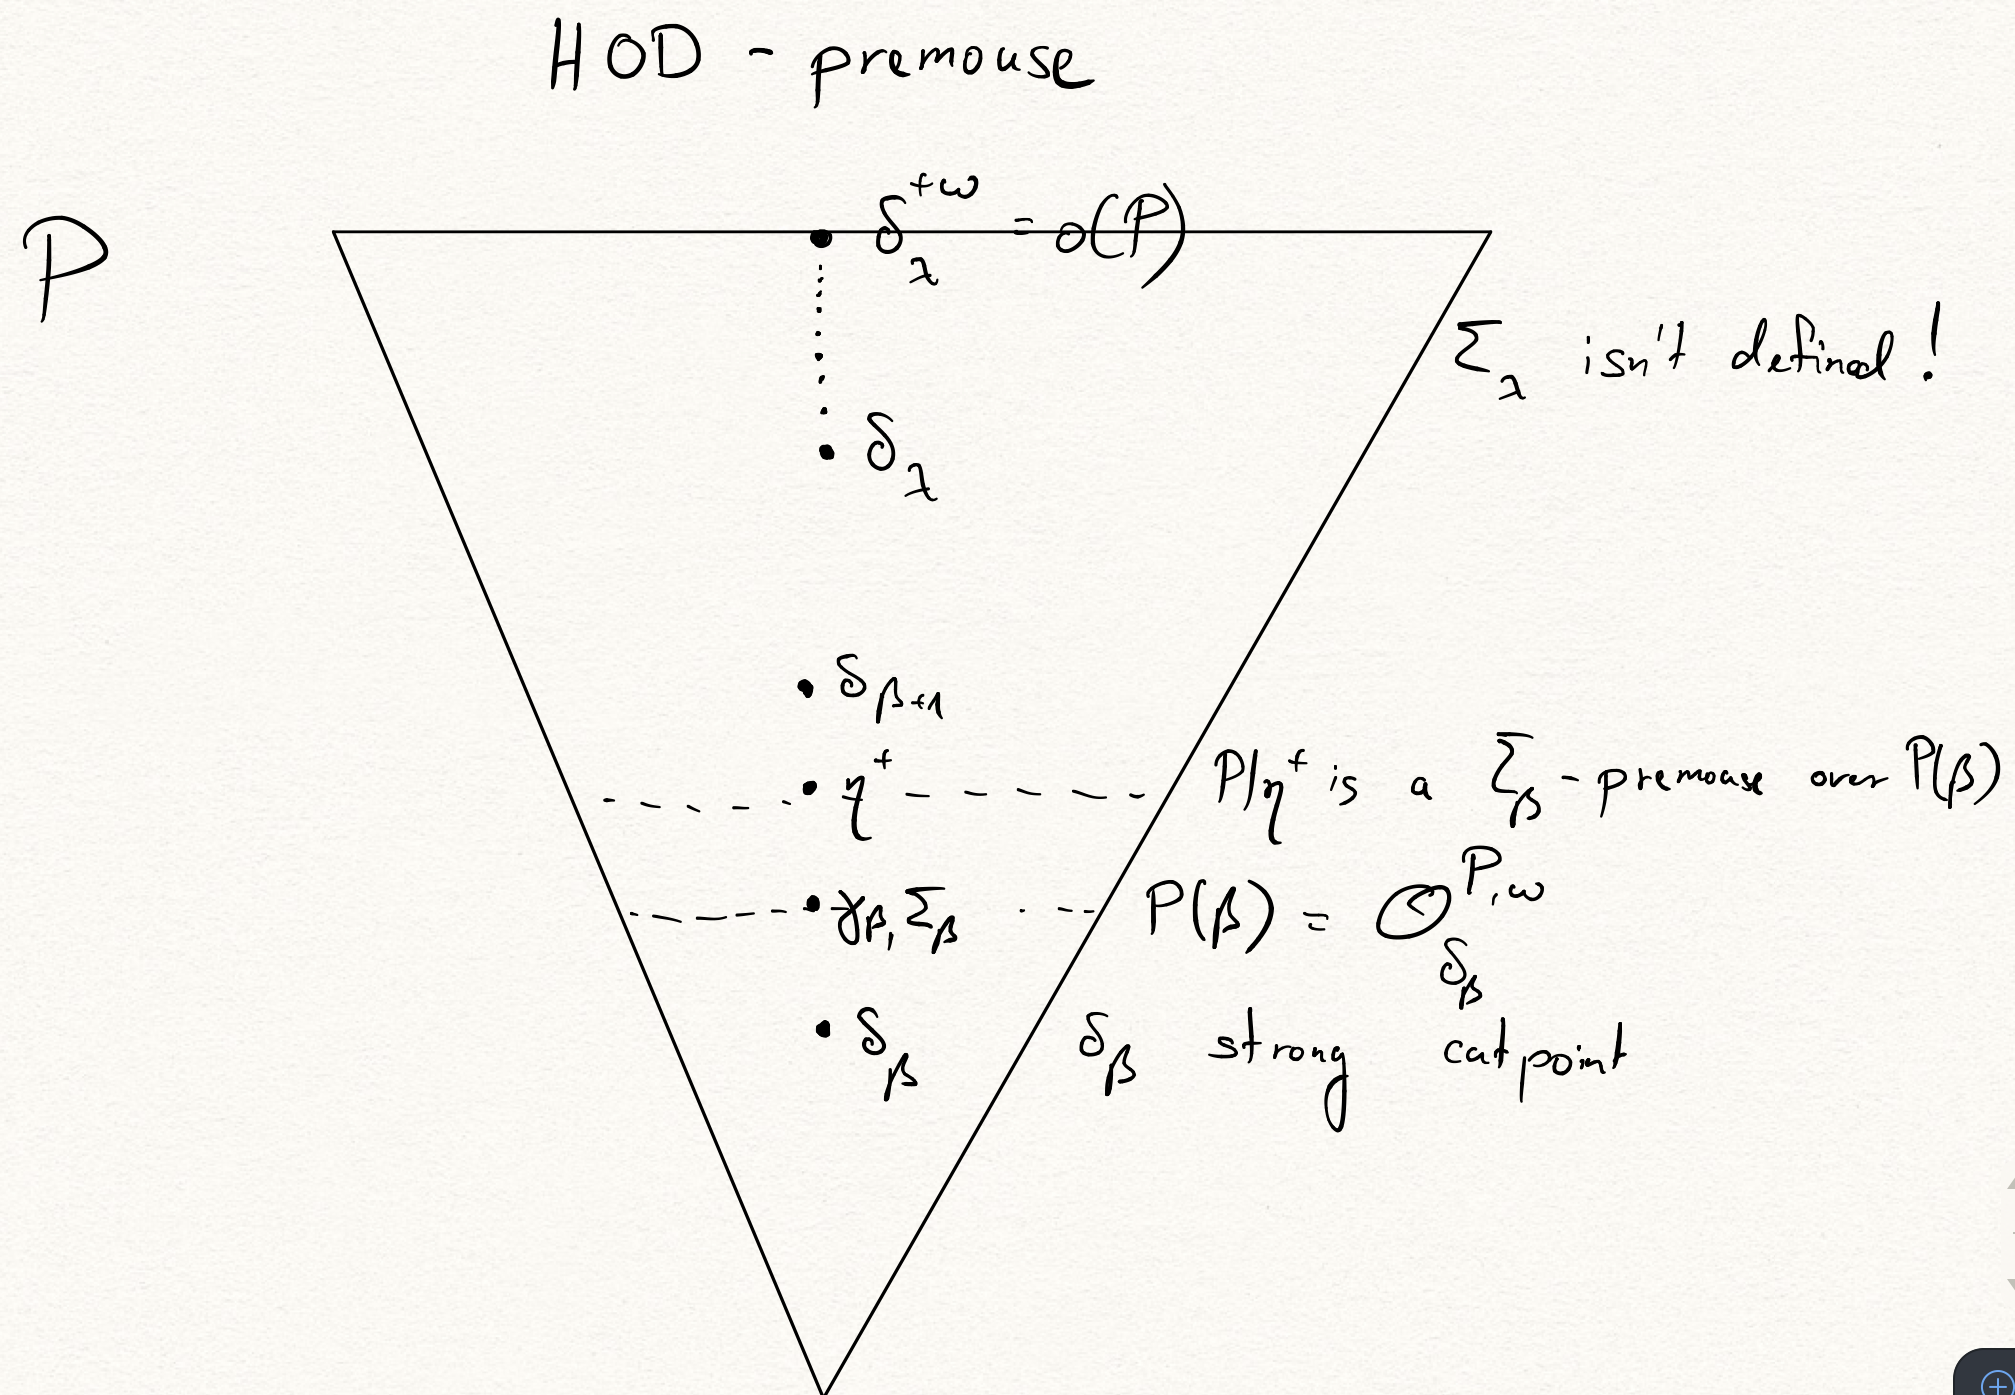
\includegraphics[width=300px]{\string~/gitsky/phd/gfx/hod-premouse.png}
  \caption{HOD premouse}
  \label{fig:hod-premouse}
\end{figure}

\defi{
  Let $\mathcal{P} = (J^{\vec{E},f}(X); \in, \vec{E}, f, B)$ be a $\hod$-premouse. We let 
  \eq{
    \mathcal{P}^{-} =
    \begin{cases}
      P | \gamma_{\lambda^{\mathcal{P}}-1} & \text{, if } \lambda^{\mathcal{P}} \text{ is a successor ordinal,} \\
      \mathcal{P}| \delta^{\mathcal{P}} & \text{, otherwise}.
    \end{cases}
  }

  See \autoref{fig:P^-}
  \todo[inline]{add picture and figure out why we don`t just let $\mathcal{P}^{-} = \mathcal{P}(\gamma^{\mathcal{P}}_{\lambda^{\mathcal{P}}-1})$ in the successor case.}
}

\begin{figure}
  \centering
  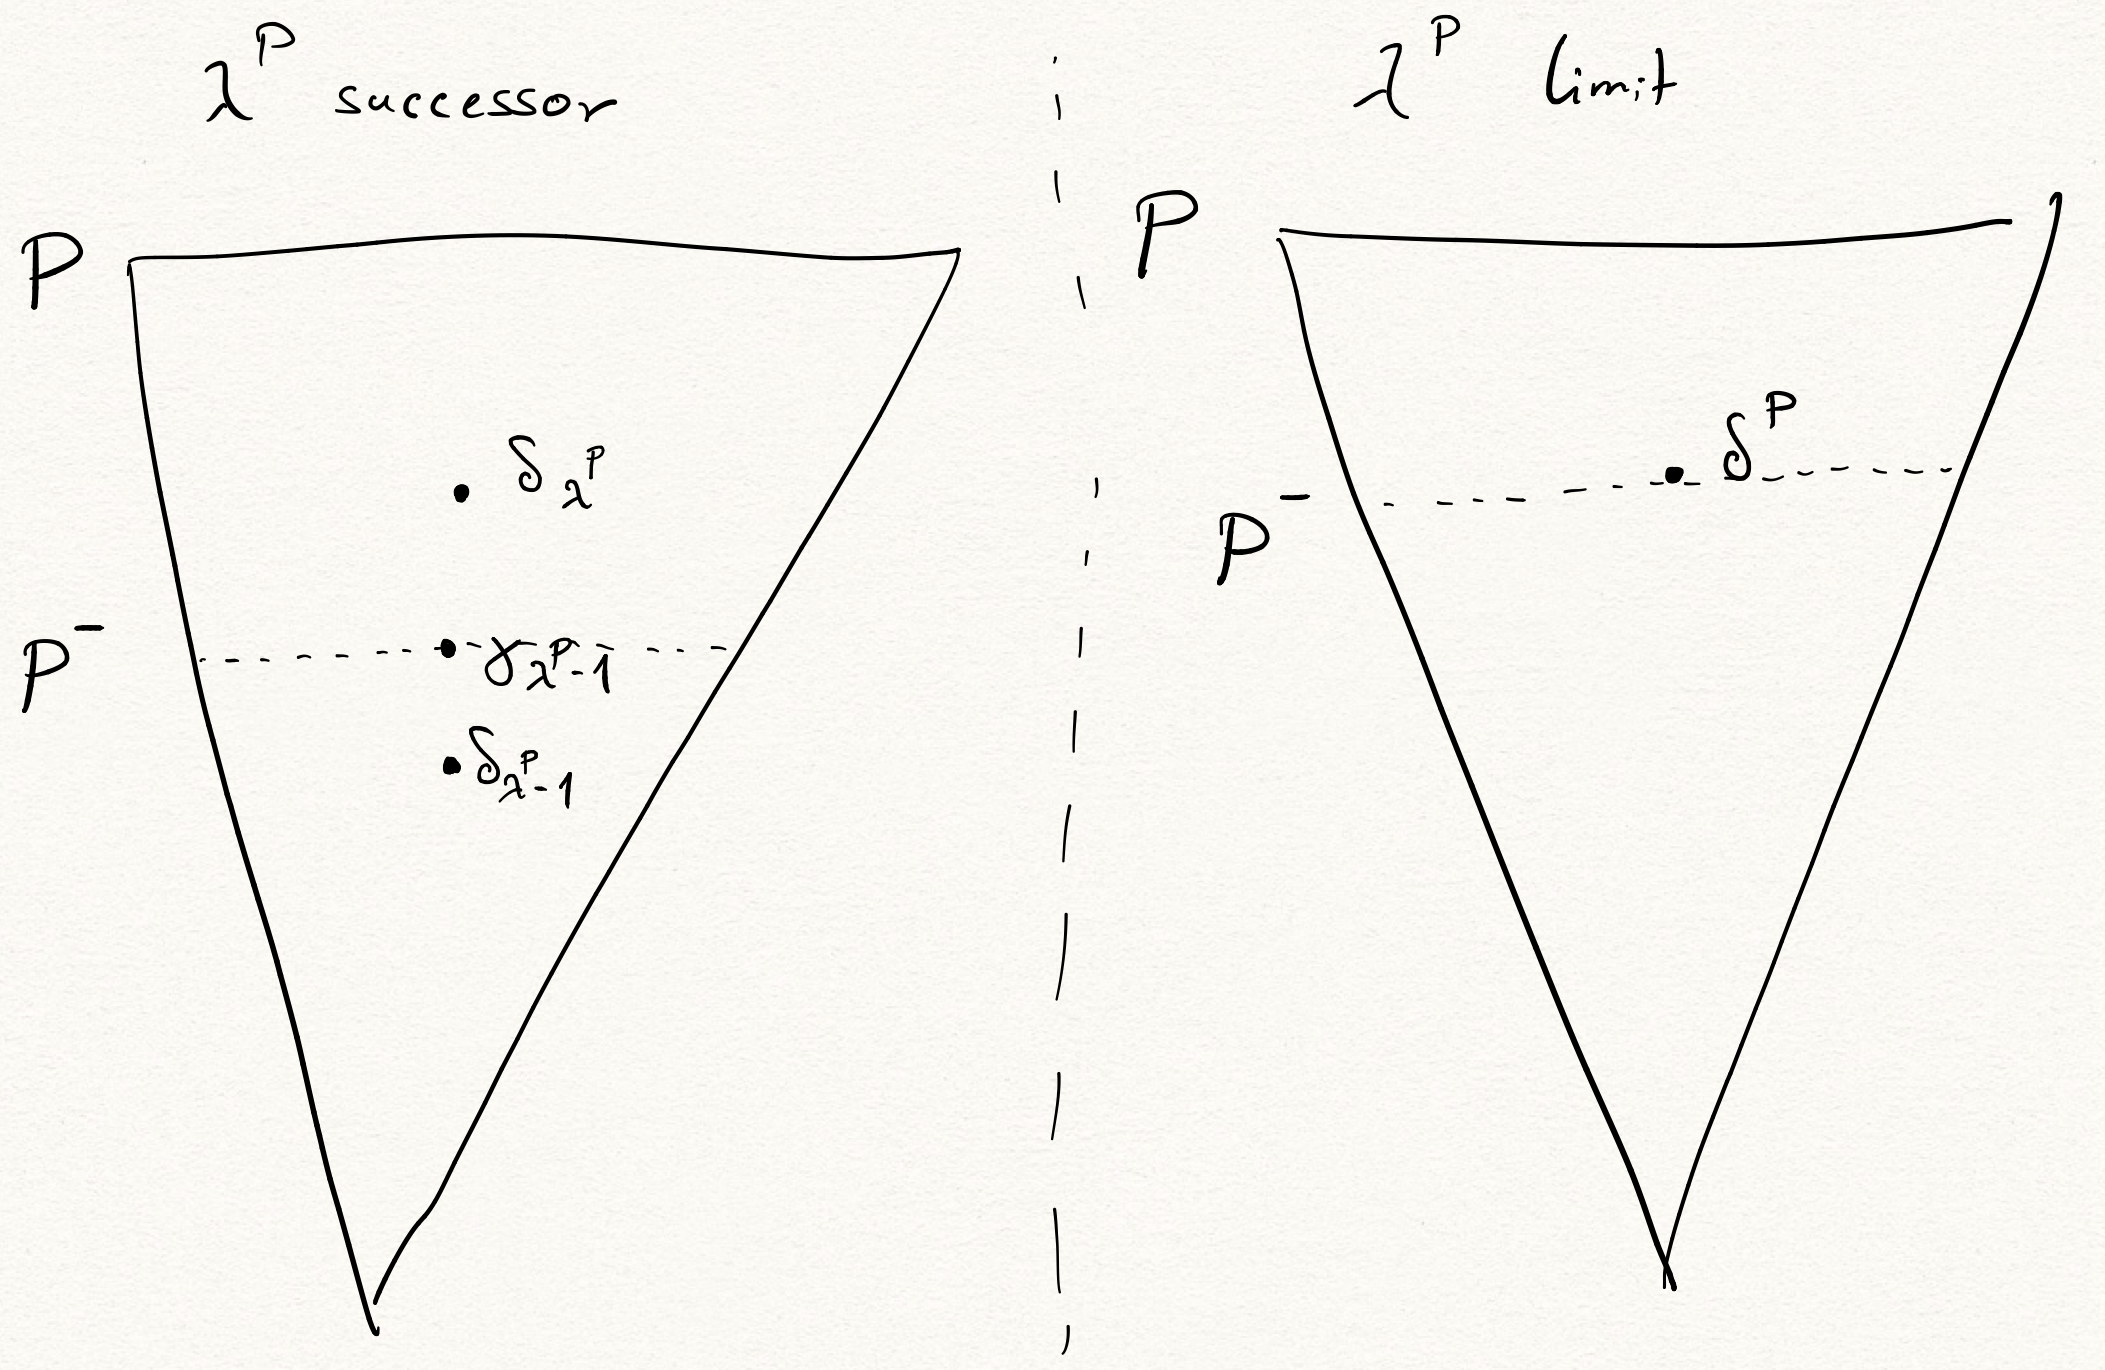
\includegraphics[width=250px]{\string~/gitsky/phd/gfx/P-minus.png}
  \caption{$\mathcal{P}^{-}$}
  \label{fig:P^-}
\end{figure}

\defi{ 
  Let $\mathcal{P}, \mathcal{Q}$ be $\hod$-premice. We write $\mathcal{P} \lehod \mathcal{Q}$ if there is some $\alpha \le \lambda^{\mathcal{Q}}$ such that $\mathcal{P} = \mathcal{Q}(\alpha)$. We also write $\mathcal{P} \lhod \mathcal{Q}$ if $\mathcal{P} \lehod \mathcal{Q}$ and $\mathcal{P} \neq \mathcal{Q}$. In this case we say that $\mathcal{P}$ is a (proper) \textbf{$\hod$-initial segment} of $\mathcal{Q}$.
}

\defi{
  Let $\mathcal{P} = (J^{\vec{E},f}(X); \in, \vec{E}, f, B)$ be a $\hod$-premouse and $\alpha \le \lambda^{\mathcal{P}}$.
  \begin{enumerate}
    \item If $\alpha < \lambda^{\mathcal{P}}$, we let $\Sigma^{\mathcal{P}}_{\alpha}$ be the internal iteration strategy of $\mathcal{P}(\alpha)$ coded by $f(\alpha)$ and
    \item $\Sigma^{\mathcal{P}}_{<\alpha} := \bigoplus_{\beta<\alpha} \Sigma^{\mathcal{P}}_{\beta}$.
  \end{enumerate}

  We also let $\Sigma^{\mathcal{P}} := \Sigma^{\mathcal{P}}_{< \lambda^{\mathcal{P}}}$.
}

\rema{
  By the agreement of the internal iteration strategies of $\hod$-premice (\autoref{defi:agreement of internal iteration strategy} in \autoref{defi:hod premouse} \todo{reference broken}), $\Sigma^{\mathcal{P}}_{\alpha}$ already includes all of the information of $\Sigma^{\mathcal{P}}_{< \alpha}$ and can be identified with $\Sigma^{\mathcal{P}}_{< \alpha + 1}$.
}

\defi{ 
  Let $\mathcal{P}$ be a $\hod$-premouse. $\Sigma$ is a \textbf{$(\kappa,\lambda)$-iteration strategy} for $\mathcal{P}$ if it is a winning strategy for player II in the iteration game $\mathcal{G}(\mathcal{P},\kappa,\lambda)$ \todo{add reference} and whenever $(\vec{\mathcal{T}},\mathcal{Q}) \in I(\mathcal{P}, \Sigma)$, then $\mathcal{Q}$ is a $\hod$-premouse such that $\Sigma^{\mathcal{Q}} = \Sigma_{\mathcal{Q}, \vec{\mathcal{T}}} \cap \mathcal{Q}$.
}

\rema{
  In particular, $\Sigma^{\mathcal{P}} = \Sigma \cap \mathcal{P}$, i.e. $\Sigma$ extends the internal iteration strategy of $\mathcal{P}$.
}

\defi{
  $(\mathcal{P}, \Sigma)$ is a \textbf{$\hod$-pair} if
  \begin{enumerate}
    \item $\mathcal{P}$ is a $\hod$-premouse and
    \item $\Sigma$ is a $(\omega_{1},\omega_{1}+1)$-iteration strategy for $\mathcal{P}$ with hull condensation.
  \end{enumerate}

  \todo[inline]{the definition of hod pair is different in both versions of Grigor`s thesis. Verify that this is the intended one.}
}

\subsection{HOD analysis}

\todo[inline]{gather all the information we need on $\hod$ -- this can be found in Grigor`s thesis}

\defi{ 
  Let $(P, \Sigma), (Q, \Lambda)$ be $\hod$-pairs. We let $(\mathcal{P}, \Sigma) \ledj (\mathcal{Q}, \Lambda)$ iff $(\mathcal{P}, \Sigma)$ loses the coiteration with $(\mathcal{Q}, \Lambda)$, i.e. there is a $(\mathcal{P}, \Sigma)$-iterate $(\mathcal{T}, R)$ and a $(\mathcal{Q}, \Lambda)$-iterate $(\mathcal{U},S)$ such that
  \eq{
    \mathcal{R} \lehod \mathcal{S} \text{ and } \Sigma_{\mathcal{R}, \mathcal{T}} = \Lambda_{\mathcal{R}, \mathcal{U}}.
  }

  We also let $(\mathcal{P}, \Sigma) \ldj (\mathcal{Q}, \Lambda)$ iff $(\mathcal{P}, \Sigma) \ledj (\mathcal{Q}, \Lambda)$ and $(\mathcal{Q}, \Lambda) \nledj (\mathcal{P}, \Sigma)$.
}

\defi{ 
  Let $(\mathcal{P}, \Sigma)$ be a $\hod$-pair such that $\Sigma$ has branch condensation and is fullness preserving. Then we define $\alpha(\P,\Sigma)$ to be the order type of $(\P, \Sigma)$ with respect to $\ledj$.
}

\rema{
  As in the case of ordinary premice, $\ledj$ (or rather $\ldj$) is a wellfounded relation. The interesting question is whether it`s total.
}

\theo[Sargsyan]{
  Assume $\ad^{+} + V = L(\mathcal{P}(\mathbb{R}))$. Suppose $(\mathcal{P}, \Sigma), (\mathcal{Q}, \Lambda)$ are $\hod$-pairs such that both $\Sigma$ and $\Lambda$ have branch condensation and are fullness preserving. Then $(\mathcal{P}, \Sigma) \ledj (\mathcal{Q}, \Lambda)$ or $(\mathcal{Q}, \Lambda) \ledj (\mathcal{P}, \Sigma)$.
}
\proof{
  \cite[Theorem~5.10]{sargsyan2015hod}.
}

\theo[Sargsyan]{ 
  Assume $\ad^{+} + V = L(\mathcal{P}(\mathbb{R}))$. Suppose $(\mathcal{P}, \Sigma), (\mathcal{Q}, \Lambda)$ are $\hod$-pairs such that both $\Sigma$ and $\Lambda$ have branch condensation and are $\Gamma$-fullness preserving for some pointclass $\Gamma$ which is closed under continuous images and preimages. Suppose further that there is a good pointclass $\Gamma^{*}$ such that $\Gamma \cup \{ \code(\Sigma), \code(\Lambda) \} \subseteq \Delta_{\underset{\sim}{\Gamma}^{*}}$ \todo{define $\code{\Sigma}$}. Then $(\mathcal{P}, \Sigma) \ledj (\mathcal{Q}, \Lambda)$ or $(\mathcal{Q}, \Lambda) \ledj (\mathcal{P}, \Sigma)$.
}
\proof{
  \cite[Theorem~2.33]{sargsyan2015hod}.
}

\defi{ 
  Suppose $\Gamma$ is a pointclass closed under Wadge reducibility and $(\mathcal{P}, \Sigma)$ is a $\hod$-pair such that $\Sigma$ has branch condensation and is $\Gamma$-fullness preserving. We let
  \begin{enumerate}
    \item $\mathcal{F}(\mathcal{P}, \Sigma) = \{ (\mathcal{Q}, \Sigma_{\mathcal{Q}}) \mid \mathcal{Q} \in pB(\mathcal{P}, \Sigma)\}$ and
    \item $\mathcal{F}^{+}(\mathcal{P}, \Sigma) = \{ (\mathcal{Q}, \Sigma_{\mathcal{Q}}) \mid \mathcal{Q} \in pI(\mathcal{P}, \Sigma)\}$.  
  \end{enumerate}
}

\rema{
  By \cite[Corollary~2.44]{sargsyan2015hod} $\Sigma$ is commuting, so that $\Sigma_{\mathcal{Q}}$ is indeed well-defined.
}

\defi{ 
  Suppose $\Gamma$ is a pointclass closed under Wadge reducibility and $(\mathcal{P}, \Sigma)$ is a $\hod$-pair such that $\Sigma$ has branch condensation and is $\Gamma$-fullness preserving. Let $\mathcal{Q}, \mathcal{R} \in pI(\mathcal{P}, \Sigma) \cup pB(\mathcal{P}, \Sigma)$. We let $\mathcal{Q} \le^{\mathcal{P},\Sigma} \mathcal{R}$ if
  \begin{enumerate}
    \item $\mathcal{Q} \in pI(\mathcal{P}, \Sigma)$ and $R \in pI(\mathcal{Q}, \Sigma_{Q})$ or
    \item $\mathcal{Q} \in pB(\mathcal{P},\Sigma)$ and $(\mathcal{Q}, \Sigma_{\mathcal{Q}}) \ledj (\mathcal{R}, \Sigma_{\mathcal{R}})$.
  \end{enumerate}
}

\lemm[Sargsyan]{
  $\le^{\mathcal{P}, \Sigma}$ is directed.
}
\proof{
  \cite[Lemma~4.17]{sargsyan2015hod}.
}


\defi{
  Suppose $\Gamma$ is a pointclass closed under Wadge reducibility and $(\mathcal{P}, \Sigma)$ is a $\hod$-pair such that $\Sigma$ has branch condensation and is $\Gamma$-fullness preserving. Let $\mathcal{Q}, \mathcal{R} \in \piterates(\mathcal{P}, \Sigma) \cup \pblowups(\mathcal{P}, \Sigma)$ be such that, for some $\alpha \le^{\mathcal{R}}$, $\mathcal{R}(\alpha) \in pI(\mathcal{Q}, \Sigma_{\mathcal{Q}})$. We let
  \eq{
    \pi^{\Sigma}_{\mathcal{Q}, \mathcal{R}} \colon \mathcal{Q} \to \mathcal{R}(\alpha)
  }

  be the iteration map given by $\Sigma_{\mathcal{Q}}$. We let
  \begin{enumerate}
    \item $\mathcal{M}_{\infty}(\mathcal{P}, \Sigma)$ be the direct limit of $\mathcal{F}(\mathcal{P},\Sigma)$ with respect to the embeddings $\pi^{\Sigma}_{\mathcal{Q}, \mathcal{R}}$ for $\mathcal{Q}, \mathcal{R} \in pB(\mathcal{P}, \Sigma)$ such that there is an $\alpha\leq\lambda^{\mathcal{R}} \mathcal{R}(\alpha) \in pI(\mathcal{Q}, \Sigma_{\mathcal{Q}}) )$; and let
    \item $\mathcal{M}^{+}_{\infty}(\mathcal{P}, \Sigma)$ be the direct limit of $\mathcal{F}(\mathcal{P},\Sigma)$ with respect to the embeddings $\pi^{\Sigma}_{\mathcal{Q}, \mathcal{R}}$ for $\mathcal{Q}, \mathcal{R} \in pI(\mathcal{P}, \Sigma)$ such that $\mathcal{Q} \leq^{\Sigma}_{\mathcal{Q}, \mathcal{R}} \mathcal{R})$.\\
  \end{enumerate}

  For $\mathcal{Q} \in pB(\mathcal{P}, \Sigma)$ and $\mathcal{R} \in pI(\mathcal{P}, \Sigma)$ we let
  \begin{enumerate}
    \item $\pi^{\Sigma}_{\mathcal{Q}, \infty} \colon \mathcal{Q} \to \mathcal{M}_{\infty}(\mathcal{P}, \Sigma)$
    \item $\sigma^{\Sigma}_{\mathcal{R}, \infty} \colon \mathcal{R} \to \mathcal{M}^{+}_{\infty}(\mathcal{P}, \Sigma)$
  \end{enumerate}

  be the direct limit maps.
}

\defi{ 
  Let $(\mathcal{P}, \Sigma)$ be as above. We let
  \begin{enumerate}
    \item $\delta_{\infty}(\mathcal{P}, \Sigma)$ be the supremum of the Woodin cardinals of $\mathcal{M}_{\infty}(\mathcal{P}, \Sigma)$,
    \item $\delta^{+}_{\infty}(\mathcal{P}, \Sigma)$ be the supremum of the Woodin cardinals of $\mathcal{M}^{+}_{\infty}(\mathcal{P}, \Sigma)$ and
    \item $\lambda_{\infty}(\mathcal{P}, \Sigma) := \lambda^{\mathcal{M}^{+}_{\infty}(\mathcal{P}, \Sigma)}$.
  \end{enumerate}  
}

\lemm[Sargsyan]{
  Let $\Gamma$ be a pointclass closed under Wadge reducibility. Suppose $(\mathcal{P}, \Sigma)$ is a $\hod$-pair such that $\lambda^{\mathcal{P}}$ is a limit ordinal and $\Sigma$ has branch condensation and is $\Gamma$-fullness preserving. Then
  \begin{enumerate}
    \item $\delta_{\infty}(\mathcal{P}, \Sigma) = \delta^{+}_{\infty}(\mathcal{P}, \Sigma)$ and
    \item $\mathcal{M}^{+}_{\infty}(\mathcal{P}, \Sigma) | \delta^{+}_{\infty} = \mathcal{M}_{\infty}(\mathcal{P}, \Sigma)$.
  \end{enumerate}
}
\proof{
  \cite[Lemma~4.18]{sargsyan2015hod}.
}

\todo[inline]{We will likely not need the entire theorem and should reduce it to the part that we need once we are done.}

\theo[Sargsyan]{
  Assume $\ad^{+}$, let $\Gamma \subseteq \mathcal{P}(\mathbb{R})$ be such that $\Gamma = \mathcal{P}(\mathbb{R}) \cap L(\Gamma, \mathbb{R})$ and $\mathcal{H} = \hod^{L(\Gamma,\mathbb{R})}$. Then the following holds:
  \begin{enumerate}
    \item If $L(\Gamma,\mathbb{R}) \models \phi$ \todo{define $\phi$} then for all $(\mathcal{P}, \Sigma) \in \Gamma$ such that $\alpha(\mathcal{P}, \Sigma) < \Omega^{\Gamma}$ \todo{define $\Omega^{\Gamma}$} we have, for all $\alpha \le \alpha(\mathcal{P}, \Sigma)$,
      \begin{enumerate}
        \item $\delta_{\alpha}^{\mathcal{M}^{+}_{\infty}(\mathcal{P}, \Sigma)} = \theta^{\Gamma}_{\alpha}$ \todo{define $\theta^{\Gamma}_{\alpha}$} and
        \item $\mathcal{M}^{+}_{\infty}(\mathcal{P}, \Sigma) | \theta^{\Gamma}_{\alpha} = (V^{\mathcal{H}}_{\theta^{\Gamma}_{\alpha}};\in, \vec{E}^{\mathcal{M}^{+}_{\infty}(\mathcal{P}, \Sigma)} \restriction \theta^{\Gamma}_{\alpha}, \Lambda \restriction \theta^{\Gamma}_{\alpha})$,
      \end{enumerate}

      where $\Lambda$ is the iteration strategy coded by $f^{\mathcal{M}^{+}_{\infty}(\mathcal{P}, \Sigma)}$.

    \item If $L(\Gamma, \mathbb{R}) \models \psi$ \todo{define $\psi$} then for all $\alpha \le \Omega^{\Gamma}$
      \begin{enumerate}
        \item $\delta_{\alpha}^{\mathcal{M}^{+}_{\infty}(\mathcal{P}, \Sigma)} = \theta^{\Gamma}_{\alpha}$ and
        \item $\mathcal{M}^{+}_{\infty}(\mathcal{P}, \Sigma) | \theta^{\Gamma}_{\alpha} = (V^{\mathcal{H}}_{\theta^{\Gamma}_{\alpha}};\in, \vec{E}^{\mathcal{M}^{+}_{\infty}(\mathcal{P}, \Sigma)} \restriction \theta^{\Gamma}_{\alpha}, \Lambda \restriction \theta^{\Gamma}_{\alpha})$.
      \end{enumerate}

    \item Suppose $\Gamma^{*} \subseteq \mathcal{P}(\mathbb{R})$ is such that $\Gamma \subseteq \Gamma^{*}$, $L(\Gamma^{*}, \mathbb{R}) \models \ad^{+}$ and there is a $\hod$-pair $(\mathcal{P}, \Sigma) \in \Gamma^{*}$ such that
      \begin{enumerate}
        \item $\Sigma$ has branch condensation and is $\Gamma$-fullness preserving,
        \item $\lambda^{\mathcal{P}}$ is a successor ordinal, $\code(\Sigma_{\mathcal{P}^{-}}) \in \Gamma$ and $L(\Gamma, \mathbb{R})$ models that $(\mathcal{P}, \Sigma_{\mathcal{P}^{-}})$ is a suitable pair such that $\alpha(\mathcal{P}^{-}, \Sigma_{\mathcal{P}^{-}}) = \alpha$, \todo{define suitable pair}
        \item there is a sequence $(B_{i} \mid i < \omega) \subseteq \mathbb{B}(\mathcal{P}^{-}, \Sigma_{\mathcal{P}^{-}})^{L(\Gamma, \mathbb{R})}$ which guides $\Sigma$ and \todo{define $\mathbb{B}(..)$ and what it means to be guided}
        \item for any $B \in \mathbb{B}(\mathcal{P}^{-}, \Sigma_{\mathcal{P}^{-}})^{L(\Gamma, \mathbb{R})}$ there is some $\mathcal{R} \in \piterates(\mathcal{P}, \Sigma)$ such that $\Sigma_{\mathcal{R}}$ respects $B$. \todo{define respects $B$}
      \end{enumerate}

      Then $L(\Gamma, \mathbb{R}) \models \psi$ and $\mathcal{M}_{\infty}(\mathcal{P}, \Sigma) = \mathcal{M}^{+}_{\infty}(\mathcal{P}, \Sigma)$.
  \end{enumerate}
}
\proof{
  \cite[Theorem~4.24]{sargsyan2015hod}.
}


\section{$\Omega$ is not zero}
\lipsum[1]

\section{$\Omega$ is not a successor}
\lipsum[1]

\section{$\Omega$ does not have countable cofinality}
\lipsum[1]

\section{$\Omega$ is not singular}
\lipsum[1]


\end{document}
